\documentclass[justified]{tufte-book}

% ams
\usepackage{amssymb,amsmath}

\usepackage{ifxetex,ifluatex}
\usepackage{fixltx2e} % provides \textsubscript
\ifnum 0\ifxetex 1\fi\ifluatex 1\fi=0 % if pdftex
  \usepackage[T1]{fontenc}
  \usepackage[utf8]{inputenc}
\else % if luatex or xelatex
  \makeatletter
  \@ifpackageloaded{fontspec}{}{\usepackage{fontspec}}
  \makeatother
  \defaultfontfeatures{Ligatures=TeX,Scale=MatchLowercase}
  \makeatletter
  \@ifpackageloaded{soul}{
     \renewcommand\allcapsspacing[1]{{\addfontfeature{LetterSpace=15}#1}}
     \renewcommand\smallcapsspacing[1]{{\addfontfeature{LetterSpace=10}#1}}
   }{}
  \makeatother

\fi

% graphix
\usepackage{graphicx}
\setkeys{Gin}{width=\linewidth,totalheight=\textheight,keepaspectratio}

% booktabs
\usepackage{booktabs}

% url
\usepackage{url}

% hyperref
\usepackage{hyperref}

% units.
\usepackage{units}


\setcounter{secnumdepth}{2}

% citations

\newlength{\cslhangindent}
\setlength{\cslhangindent}{1.5em}
% For Pandoc 2.8 to 2.11
\newenvironment{cslreferences}%
  {}%
  {\par}
% For pandoc 2.11+ using new --citeproc
\newlength{\csllabelwidth}
\setlength{\csllabelwidth}{3em}
\newlength{\cslentryspacingunit} % times entry-spacing
\setlength{\cslentryspacingunit}{\parskip}
\newenvironment{CSLReferences}[2] % #1 hanging-ident, #2 entry spacing
 {% don't indent paragraphs
  \setlength{\parindent}{0pt}
  % turn on hanging indent if param 1 is 1
  \ifodd #1
  \let\oldpar\par
  \def\par{\hangindent=\cslhangindent\oldpar}
  \fi
  % set entry spacing
  \setlength{\parskip}{#2\cslentryspacingunit}
 }%
 {}
\usepackage{calc}
\newcommand{\CSLBlock}[1]{#1\hfill\break}
\newcommand{\CSLLeftMargin}[1]{\parbox[t]{\csllabelwidth}{#1}}
\newcommand{\CSLRightInline}[1]{\parbox[t]{\linewidth - \csllabelwidth}{#1}}
\newcommand{\CSLIndent}[1]{\hspace{\cslhangindent}#1}

% pandoc syntax highlighting
\usepackage{color}
\usepackage{fancyvrb}
\newcommand{\VerbBar}{|}
\newcommand{\VERB}{\Verb[commandchars=\\\{\}]}
\DefineVerbatimEnvironment{Highlighting}{Verbatim}{commandchars=\\\{\}}
% Add ',fontsize=\small' for more characters per line
\newenvironment{Shaded}{}{}
\newcommand{\AlertTok}[1]{\textcolor[rgb]{1.00,0.00,0.00}{\textbf{#1}}}
\newcommand{\AnnotationTok}[1]{\textcolor[rgb]{0.38,0.63,0.69}{\textbf{\textit{#1}}}}
\newcommand{\AttributeTok}[1]{\textcolor[rgb]{0.49,0.56,0.16}{#1}}
\newcommand{\BaseNTok}[1]{\textcolor[rgb]{0.25,0.63,0.44}{#1}}
\newcommand{\BuiltInTok}[1]{#1}
\newcommand{\CharTok}[1]{\textcolor[rgb]{0.25,0.44,0.63}{#1}}
\newcommand{\CommentTok}[1]{\textcolor[rgb]{0.38,0.63,0.69}{\textit{#1}}}
\newcommand{\CommentVarTok}[1]{\textcolor[rgb]{0.38,0.63,0.69}{\textbf{\textit{#1}}}}
\newcommand{\ConstantTok}[1]{\textcolor[rgb]{0.53,0.00,0.00}{#1}}
\newcommand{\ControlFlowTok}[1]{\textcolor[rgb]{0.00,0.44,0.13}{\textbf{#1}}}
\newcommand{\DataTypeTok}[1]{\textcolor[rgb]{0.56,0.13,0.00}{#1}}
\newcommand{\DecValTok}[1]{\textcolor[rgb]{0.25,0.63,0.44}{#1}}
\newcommand{\DocumentationTok}[1]{\textcolor[rgb]{0.73,0.13,0.13}{\textit{#1}}}
\newcommand{\ErrorTok}[1]{\textcolor[rgb]{1.00,0.00,0.00}{\textbf{#1}}}
\newcommand{\ExtensionTok}[1]{#1}
\newcommand{\FloatTok}[1]{\textcolor[rgb]{0.25,0.63,0.44}{#1}}
\newcommand{\FunctionTok}[1]{\textcolor[rgb]{0.02,0.16,0.49}{#1}}
\newcommand{\ImportTok}[1]{#1}
\newcommand{\InformationTok}[1]{\textcolor[rgb]{0.38,0.63,0.69}{\textbf{\textit{#1}}}}
\newcommand{\KeywordTok}[1]{\textcolor[rgb]{0.00,0.44,0.13}{\textbf{#1}}}
\newcommand{\NormalTok}[1]{#1}
\newcommand{\OperatorTok}[1]{\textcolor[rgb]{0.40,0.40,0.40}{#1}}
\newcommand{\OtherTok}[1]{\textcolor[rgb]{0.00,0.44,0.13}{#1}}
\newcommand{\PreprocessorTok}[1]{\textcolor[rgb]{0.74,0.48,0.00}{#1}}
\newcommand{\RegionMarkerTok}[1]{#1}
\newcommand{\SpecialCharTok}[1]{\textcolor[rgb]{0.25,0.44,0.63}{#1}}
\newcommand{\SpecialStringTok}[1]{\textcolor[rgb]{0.73,0.40,0.53}{#1}}
\newcommand{\StringTok}[1]{\textcolor[rgb]{0.25,0.44,0.63}{#1}}
\newcommand{\VariableTok}[1]{\textcolor[rgb]{0.10,0.09,0.49}{#1}}
\newcommand{\VerbatimStringTok}[1]{\textcolor[rgb]{0.25,0.44,0.63}{#1}}
\newcommand{\WarningTok}[1]{\textcolor[rgb]{0.38,0.63,0.69}{\textbf{\textit{#1}}}}

% table with pandoc
\usepackage{longtable,booktabs,array}
\usepackage{calc} % for calculating minipage widths
% Correct order of tables after \paragraph or \subparagraph
\usepackage{etoolbox}
\makeatletter
\patchcmd\longtable{\par}{\if@noskipsec\mbox{}\fi\par}{}{}
\makeatother
% Allow footnotes in longtable head/foot
\IfFileExists{footnotehyper.sty}{\usepackage{footnotehyper}}{\usepackage{footnote}}
\makesavenoteenv{longtable}

% multiplecol
\usepackage{multicol}

% strikeout
\usepackage[normalem]{ulem}

% morefloats
\usepackage{morefloats}


% tightlist macro required by pandoc >= 1.14
\providecommand{\tightlist}{%
  \setlength{\itemsep}{0pt}\setlength{\parskip}{0pt}}

% title / author / date
\title{Topics in Empirical Finance}
\author{Patrick Hénaff}
\date{}

%\usepackage{fontspec}
% Preamble from Rmetrics

\usepackage{booktabs}
\usepackage{amsthm}
\makeatletter
\def\thm@space@setup{%
  \thm@preskip=8pt plus 2pt minus 4pt
  \thm@postskip=\thm@preskip
}
\makeatother

% Index
\usepackage{makeidx}
\makeindex

% binomial trees
\usepackage{pgfplots}
\usepackage{tikz}
\usetikzlibrary{shapes}
\usetikzlibrary{external}
\usepgfplotslibrary{external}

% R and other languages

\newcommand{\RR}{\textsf{R}}
\newcommand{\Rmetrics}{Rmetrics}

\newcommand{\Rfun}[1]{\texttt{#1()}\index{R~functions@\RR~functions!#1}}
\newcommand{\class}[1]{\texttt{#1}}
%\newcommand{\class}[1]{\texttt{#1}\index{R~classes@\RR~classes!#1}}
\newcommand{\pkg}[1]{\texttt{#1}\index{R~packages@\RR~packages!#1}}
\newcommand{\dataset}[1]{\texttt{#1}\index{R~data@\RR~data!#1}}
\newcommand{\code}[1]{\texttt{#1}\index{#1}}

% Preamble from VIP

\newcommand{\given}{\mid}
\renewcommand{\neg}{\mathbin{\sim}}
\renewcommand{\wedge}{\mathbin{\&}}
\renewcommand{\u}{U}
\newcommand{\gt}{>}
\newcommand{\p}{Pr}
\newcommand{\E}{E}
\newcommand{\EU}{EU}
\newcommand{\pr}{Pr}
\newcommand{\po}{Pr^*}
\newcommand{\degr}{^{\circ}}
\definecolor{bookred}{RGB}{228,6,19}
\definecolor{bookblue}{RGB}{0,92,169}
\definecolor{bookpurple}{RGB}{114,49,94}

\newenvironment{epigraph}%
{
\begin{flushright}    
\begin{minipage}{20em}
\begin{flushright}
\itshape
}%
{
\end{flushright}
\end{minipage}
\end{flushright}
}
\newenvironment{problem}{\begin{quote}\normalsize}{\end{quote}}
\newenvironment{puzzle}{\begin{quote}\normalsize}{\end{quote}}
\def\argument{\list{}{\leftmargin3em}\item[]}
\let\endargument=\endlist 
\usepackage{fontawesome}
\newenvironment{warning}{\begin{itemize}\item[\faBan]}{\end{itemize}}
\usepackage{marvosym}
\newenvironment{info}{\begin{itemize}\item[\Info]}{\end{itemize}}

%%%% Kevin Godny's code for title page and contents from https://groups.google.com/forum/#!topic/tufte-latex/ujdzrktC1BQ
\makeatletter
\renewcommand{\maketitlepage}{%
\begingroup%
\setlength{\parindent}{0pt}
{\fontsize{18}{18}\selectfont\textit{\@author}\par}
\vspace{1.75in}{\fontsize{36}{14}\selectfont\@title\par}
\vspace{0.5in}{\fontsize{20}{14}\selectfont with R and Rmetrics\par}
\vspace{0.5in}{\fontsize{14}{14}\selectfont\textsf{\smallcaps{v 0.1}}\par}
\vfill{\fontsize{14}{14}\selectfont\textit{An Open Access Publication}\par}
\thispagestyle{empty}
\endgroup
}
\makeatother

% Change shape from [display] to [block] to keep chapter numbers and titles on the same line
\titleformat{\chapter}%
  [block]% shape
  {\relax\ifthenelse{\NOT\boolean{@tufte@symmetric}}{\begin{fullwidth}}{}}% format applied to label+text
  {\itshape\huge\thechapter}% label
  {3em}% horizontal separation between label and title body
  {\huge\rmfamily\itshape}% before the title body
  [\ifthenelse{\NOT\boolean{@tufte@symmetric}}{\end{fullwidth}}{}]% after the title body


\usepackage{etoolbox}
% Jesse Rosenthal's code from https://groups.google.com/forum/#!topic/pandoc-discuss/wCF78X6SvwY
% Avoid new pagraph/indent after lists, quotes, etc.
\makeatletter
\newcommand{\gobblepars}{% 
    \@ifnextchar\par% 
        {\expandafter\gobblepars\@gobble}% 
        {}}
\newcommand{\eatpar}{\@ifnextchar\par{\@gobble}{}}
\newcommand{\forcepar}{\par}
\makeatother
\AfterEndEnvironment{quote}{\expandafter\gobblepars}
\AfterEndEnvironment{enumerate}{\expandafter\gobblepars}
\AfterEndEnvironment{itemize}{\expandafter\gobblepars}
\AfterEndEnvironment{description}{\expandafter\gobblepars}
\AfterEndEnvironment{example}{\expandafter\gobblepars}
\AfterEndEnvironment{argument}{\expandafter\gobblepars}
\AfterEndEnvironment{problem}{\expandafter\gobblepars}
\AfterEndEnvironment{info}{\expandafter\gobblepars}
\AfterEndEnvironment{warning}{\expandafter\gobblepars}
\AfterEndEnvironment{marginfigure}{\expandafter\gobblepars}
\AfterEndEnvironment{longtable}{\expandafter\gobblepars} % not working, why?
\makeatletter
\AfterEndEnvironment{longtable}{\par\@afterindentfalse\@afterheading} % this seems to work instead
\makeatother

\renewcommand*\descriptionlabel[1]{\hspace\labelsep\normalfont\em #1.}

% prevent extra space when \newthought follows \section
% see: https://tex.stackexchange.com/questions/291746/tufte-latex-newthought-after-section
\makeatletter
\def\tuftebreak{%
  \if@nobreak\else
    \par
    \ifdim\lastskip<\tufteskipamount
      \removelastskip \penalty -100
      \tufteskip
    \fi
  \fi
}
\makeatother

% indent lists a bit
\usepackage{enumitem}
\setlist[1]{leftmargin=24pt}

\def\labelitemii{$\circ$}

\begin{document}

\maketitle



{
\setcounter{tocdepth}{0}
\tableofcontents
}

\hypertarget{preface}{%
\chapter*{Preface}\label{preface}}
\addcontentsline{toc}{chapter}{Preface}

\newthought{This} textbook is about empirical finance, and focusses on the pricing and risk management of financial assets: bonds, futures contracts, and other derivative securities.

The emphasis of this text is empirical. We present models, and verify their relevance by testing them of real data. We emphasize:

\begin{itemize}
\item an incremental approach to model building, starting from simple models, and building upon that foundation to construct more complex models, as needed,
\item a data-driven approach: we will implement all the models that are presented, using the R statistical package and the Rmetrics libraries,
\item the systematic use of simulation as a way of validating modeling decisions.
\end{itemize}

Last but not least, a particular attention is given to model estimation, in order to measure the tradeoff between model complexity and the challenges of a robust calibration.

This course would not be possible without the \RR{} statistical program and without the Rmetrics packages. We extend our deep appreciation to the \RR{} community and to Diethelm Wuertz and the Rmetrics team.

This book is open access (free as in free beer). It's also \href{https://github.com/phenaff/empirical-finance-2}{open source}: feel free to clone and submit additions.
You can download a \href{https://github.com/phenaff/empirical-finance-2/docs/empiricalfin.pdf}{PDF copy}

\hypertarget{part-computational-framework}{%
\part*{Computational Framework}\label{part-computational-framework}}
\addcontentsline{toc}{part}{Computational Framework}

This first part is dedicated to the description of the experimental
environment used in this book.

As mentioned earlier, our approach is data-driven and empirical. It is
thus appropriate to start this text with a description of the sources of
data that we will use, and how to fetch publicly available financial
data from the Internet.

In the following chapters, we will make repeated use of the Rmetrics
pricing libraries, and often compare different models applied to the
same data. To facilitate this comparison, the Rmetrics pricing libraries
have been wrapped in a object-oriented framework, which hides most of
the implementation details, and allows us to focus on the key features
of the financial instruments and models. The framework uses the S4
object model (\protect\hyperlink{ref-Genolini2008}{\textbf{Genolini2008?}}) of the R language, and is described in
Chapter \ref{basic-components}.

Simulation is our tool of choice to explore the features of pricing
models and test their robustness. To that end, we have developped a
framework that facilitates the definition and testing of simple risk
management strategies. The core of this simulation framework is the \class{DataProvider}
class, which is presented in Chapter \ref{sim-framework}.

In addition to the packages found on CRAN, data sets and code used in the
text have been gathered into three packages:

\begin{description}
\tightlist
\item[empfin]
contains all the data sets and several utility functions for simple bond pricing and the manipulation of dates,
\item[fInstrument]
provides the \class{fInstrument} class, that wraps the Rmetrics pricing library and the \class{DataProvider} class, that acts as a container for market data,
\item[DynamicSimulation]
contains tools needed to perform dynamic simulations, such as scenario generators and delta hedging simulators.
\end{description}

\hypertarget{basic-components}{%
\chapter{Basic Components}\label{basic-components}}

\begin{Shaded}
\begin{Highlighting}[]
\FunctionTok{library}\NormalTok{(fOptions)}
\FunctionTok{library}\NormalTok{(fExoticOptions)}
\FunctionTok{library}\NormalTok{(fInstrument)}
\FunctionTok{library}\NormalTok{(DynamicSimulation)}
\FunctionTok{library}\NormalTok{(empfin)}
\FunctionTok{library}\NormalTok{(plotly)}
\end{Highlighting}
\end{Shaded}

This chapter provides a tutorial and explains the design of the object framework that has been build on top of the Rmetrics library.
As mentioned earlier, this layer is meant to hide
most of the implementation details, and allows us to focus on the key features of the
financial instruments and models.

The reader is encouraged to work through the examples, but the sections on design and implementation can be skipped.

The object framework involves two main entities:

\begin{itemize}
\tightlist
\item
  the \class{fInstrument} class models an abstract financial instrument, and exposes
  generic methods for computing the net present value (NPV) and the risk
  indicators (the ``greeks'\,'). With this class, one can perform calculations on portfolio of instruments, without being concerned about the implementation details specific to each type of asset. This will be illustrated below with the detailed description of a delta-hedging algorithm.
\item
  the \class{DataProvider} class is a container for market data, derived from the built-in \RR{} \code{environment}. It greatly simplifies the signature of pricing functions. Instead of passing as arguments all the necessary market data, we simply pass one \class{DataProvider} argument. The pricing methods fetch the necessary data from the \class{DataProvider}, as needed.
\end{itemize}

Each entity is now described and illustrated.

\hypertarget{the-class}{%
\section{\texorpdfstring{The \class{fInstrument} Class}{The  Class}}\label{the-class}}

As mentioned, the purpose of the \class{fInstrument} class is to create a layer of abstraction over the large variety of pricing models found in Rmetrics. With this class, we can express calculation algorithms in a generic manner. This is best explained by an example.

\hypertarget{illustration}{%
\subsection{Illustration}\label{illustration}}

Consider a portfolio made of two options, a vanilla European call and a binary (cash-or-nothing) option, both written on the same underlying asset. We would like to compute the NPV and delta of this portfolio. Let's contrast the process, first performed with the Rmetrics functions, and then with the \class{fInstrument} class.

Starting with the Rmetrics functions, you first compute the price and delta of the European call:

\begin{Shaded}
\begin{Highlighting}[]
\NormalTok{p }\OtherTok{\textless{}{-}} \FunctionTok{vector}\NormalTok{(}\AttributeTok{mode =} \StringTok{"numeric"}\NormalTok{, }\AttributeTok{length =} \DecValTok{2}\NormalTok{)}
\NormalTok{d }\OtherTok{\textless{}{-}} \FunctionTok{vector}\NormalTok{(}\AttributeTok{mode =} \StringTok{"numeric"}\NormalTok{, }\AttributeTok{length =} \DecValTok{2}\NormalTok{)}
\end{Highlighting}
\end{Shaded}

\begin{Shaded}
\begin{Highlighting}[]
\NormalTok{p }\OtherTok{\textless{}{-}} \FunctionTok{vector}\NormalTok{(}\AttributeTok{mode =} \StringTok{"numeric"}\NormalTok{, }\AttributeTok{length =} \DecValTok{2}\NormalTok{)}
\NormalTok{cp }\OtherTok{\textless{}{-}} \StringTok{"c"}
\NormalTok{Spot }\OtherTok{\textless{}{-}} \DecValTok{100}
\NormalTok{Strike }\OtherTok{\textless{}{-}} \DecValTok{100}
\NormalTok{Ttm }\OtherTok{\textless{}{-}} \DecValTok{1}
\NormalTok{int.rate }\OtherTok{\textless{}{-}} \FloatTok{0.02}
\NormalTok{div.yield }\OtherTok{\textless{}{-}} \FloatTok{0.02}
\NormalTok{sigma }\OtherTok{\textless{}{-}} \FloatTok{0.3}
\NormalTok{p[}\DecValTok{1}\NormalTok{] }\OtherTok{\textless{}{-}} \FunctionTok{GBSOption}\NormalTok{(}\AttributeTok{TypeFlag =}\NormalTok{ cp, }\AttributeTok{S =}\NormalTok{ Spot, }\AttributeTok{X =}\NormalTok{ Strike,}
    \AttributeTok{Time =}\NormalTok{ Ttm, }\AttributeTok{r =}\NormalTok{ int.rate, }\AttributeTok{b =}\NormalTok{ int.rate }\SpecialCharTok{{-}}\NormalTok{ div.yield,}
    \AttributeTok{sigma =}\NormalTok{ sigma)}\SpecialCharTok{@}\NormalTok{price}
\NormalTok{d[}\DecValTok{1}\NormalTok{] }\OtherTok{\textless{}{-}} \FunctionTok{GBSGreeks}\NormalTok{(}\AttributeTok{Selection =} \StringTok{"delta"}\NormalTok{, }\AttributeTok{TypeFlag =}\NormalTok{ cp,}
    \AttributeTok{S =}\NormalTok{ Spot, }\AttributeTok{X =}\NormalTok{ Strike, }\AttributeTok{Time =}\NormalTok{ Ttm, }\AttributeTok{r =}\NormalTok{ int.rate,}
    \AttributeTok{b =}\NormalTok{ int.rate }\SpecialCharTok{{-}}\NormalTok{ div.yield, }\AttributeTok{sigma =}\NormalTok{ sigma)}
\end{Highlighting}
\end{Shaded}

Perform the same calculation for the binary option. The delta is computed
by finite difference.

\begin{Shaded}
\begin{Highlighting}[]
\NormalTok{p }\OtherTok{\textless{}{-}} \FunctionTok{vector}\NormalTok{(}\AttributeTok{mode =} \StringTok{"numeric"}\NormalTok{, }\AttributeTok{length =} \DecValTok{2}\NormalTok{)}
\NormalTok{K }\OtherTok{\textless{}{-}} \DecValTok{1}
\NormalTok{p[}\DecValTok{2}\NormalTok{] }\OtherTok{\textless{}{-}} \FunctionTok{CashOrNothingOption}\NormalTok{(}\AttributeTok{TypeFlag =}\NormalTok{ cp, }\AttributeTok{S =}\NormalTok{ Spot,}
    \AttributeTok{X =}\NormalTok{ Strike, }\AttributeTok{K =}\NormalTok{ K, }\AttributeTok{Time =}\NormalTok{ Ttm, }\AttributeTok{r =}\NormalTok{ int.rate, }\AttributeTok{b =}\NormalTok{ int.rate }\SpecialCharTok{{-}}
\NormalTok{        div.yield, }\AttributeTok{sigma =}\NormalTok{ sigma)}\SpecialCharTok{@}\NormalTok{price}
\NormalTok{h }\OtherTok{\textless{}{-}}\NormalTok{ Spot }\SpecialCharTok{*} \FloatTok{0.001}
\NormalTok{dh }\OtherTok{\textless{}{-}} \FunctionTok{CashOrNothingOption}\NormalTok{(}\AttributeTok{TypeFlag =}\NormalTok{ cp, }\AttributeTok{S =} \FunctionTok{c}\NormalTok{(Spot }\SpecialCharTok{+}
\NormalTok{    h, Spot }\SpecialCharTok{{-}}\NormalTok{ h), }\AttributeTok{X =}\NormalTok{ Strike, }\AttributeTok{K =}\NormalTok{ K, }\AttributeTok{Time =}\NormalTok{ Ttm, }\AttributeTok{r =}\NormalTok{ int.rate,}
    \AttributeTok{b =}\NormalTok{ int.rate }\SpecialCharTok{{-}}\NormalTok{ div.yield, }\AttributeTok{sigma =}\NormalTok{ sigma)}\SpecialCharTok{@}\NormalTok{price}
\NormalTok{d[}\DecValTok{2}\NormalTok{] }\OtherTok{\textless{}{-}} \FunctionTok{diff}\NormalTok{(dh)}\SpecialCharTok{/}\NormalTok{(}\DecValTok{2} \SpecialCharTok{*}\NormalTok{ h)}
\end{Highlighting}
\end{Shaded}

Finally, sum both vectors to get the portfolio NPV and delta.

\begin{Shaded}
\begin{Highlighting}[]
\NormalTok{p }\OtherTok{\textless{}{-}} \FunctionTok{vector}\NormalTok{(}\AttributeTok{mode =} \StringTok{"numeric"}\NormalTok{, }\AttributeTok{length =} \DecValTok{2}\NormalTok{)}
\FunctionTok{print}\NormalTok{(}\FunctionTok{paste}\NormalTok{(}\StringTok{"Price:"}\NormalTok{, }\FunctionTok{round}\NormalTok{(}\FunctionTok{sum}\NormalTok{(p), }\DecValTok{2}\NormalTok{), }\StringTok{"Delta:"}\NormalTok{, }\FunctionTok{round}\NormalTok{(}\FunctionTok{sum}\NormalTok{(d),}
    \DecValTok{3}\NormalTok{)))}
\end{Highlighting}
\end{Shaded}

\begin{verbatim}
## [1] "Price: 0 Delta: 0.536"
\end{verbatim}

With the \class{fInstrument} class, the calculation steps are quite different.

You first create a vanilla instrument with the \code{fInstrumentFactory} function:

\begin{Shaded}
\begin{Highlighting}[]
\NormalTok{dtExpiry }\OtherTok{\textless{}{-}} \FunctionTok{myDate}\NormalTok{(}\StringTok{"01jan2011"}\NormalTok{)}
\NormalTok{underlying }\OtherTok{\textless{}{-}} \StringTok{"IBM"}
\NormalTok{Strike }\OtherTok{\textless{}{-}} \DecValTok{100}
\NormalTok{K }\OtherTok{\textless{}{-}} \DecValTok{1}

\NormalTok{b }\OtherTok{\textless{}{-}} \FunctionTok{fInstrumentFactory}\NormalTok{(}\StringTok{"vanilla"}\NormalTok{, }\AttributeTok{quantity =} \DecValTok{1}\NormalTok{, }\AttributeTok{params =} \FunctionTok{list}\NormalTok{(}\AttributeTok{cp =} \StringTok{"c"}\NormalTok{,}
    \AttributeTok{strike =}\NormalTok{ Strike, }\AttributeTok{dtExpiry =}\NormalTok{ dtExpiry, }\AttributeTok{underlying =}\NormalTok{ underlying,}
    \AttributeTok{discountRef =} \StringTok{"USD.LIBOR"}\NormalTok{, }\AttributeTok{trace =} \ConstantTok{FALSE}\NormalTok{))}
\end{Highlighting}
\end{Shaded}

Next, use again the \code{fInstrumentfactory} to create the binary option:

\begin{Shaded}
\begin{Highlighting}[]
\NormalTok{v }\OtherTok{\textless{}{-}} \FunctionTok{fInstrumentFactory}\NormalTok{(}\StringTok{"binary"}\NormalTok{, }\AttributeTok{quantity =} \DecValTok{1}\NormalTok{, }\AttributeTok{params =} \FunctionTok{list}\NormalTok{(}\AttributeTok{cp =} \StringTok{"c"}\NormalTok{,}
    \AttributeTok{strike =}\NormalTok{ Strike, }\AttributeTok{dtExpiry =}\NormalTok{ dtExpiry, }\AttributeTok{K =}\NormalTok{ K, }\AttributeTok{underlying =}\NormalTok{ underlying,}
    \AttributeTok{discountRef =} \StringTok{"USD.LIBOR"}\NormalTok{, }\AttributeTok{trace =} \ConstantTok{FALSE}\NormalTok{))}
\end{Highlighting}
\end{Shaded}

Insert the relevant market data into a \class{DataProvider} (this will be explained in the next section):

\begin{Shaded}
\begin{Highlighting}[]
\NormalTok{base.env }\OtherTok{\textless{}{-}} \FunctionTok{DataProvider}\NormalTok{()}
\NormalTok{dtCalc }\OtherTok{\textless{}{-}} \FunctionTok{myDate}\NormalTok{(}\StringTok{"01jan2010"}\NormalTok{)}
\FunctionTok{setData}\NormalTok{(base.env, underlying, }\StringTok{"Price"}\NormalTok{, dtCalc, }\DecValTok{100}\NormalTok{)}
\FunctionTok{setData}\NormalTok{(base.env, underlying, }\StringTok{"DivYield"}\NormalTok{, dtCalc, div.yield)}
\FunctionTok{setData}\NormalTok{(base.env, underlying, }\StringTok{"ATMVol"}\NormalTok{, dtCalc, sigma)}
\FunctionTok{setData}\NormalTok{(base.env, }\StringTok{"USD.LIBOR"}\NormalTok{, }\StringTok{"Yield"}\NormalTok{, dtCalc, int.rate)}
\end{Highlighting}
\end{Shaded}

Construct a portfolio, as a list of \class{fInstrument} objects:

\begin{Shaded}
\begin{Highlighting}[]
\NormalTok{portfolio }\OtherTok{=} \FunctionTok{c}\NormalTok{(v, b)}
\end{Highlighting}
\end{Shaded}

and finally compute the price and delta of the portfolio:

\begin{Shaded}
\begin{Highlighting}[]
\NormalTok{price }\OtherTok{\textless{}{-}} \FunctionTok{sum}\NormalTok{(}\FunctionTok{sapply}\NormalTok{(portfolio, }\ControlFlowTok{function}\NormalTok{(a) }\FunctionTok{getValue}\NormalTok{(a,}
    \StringTok{"Price"}\NormalTok{, dtCalc, base.env)))}
\NormalTok{delta }\OtherTok{\textless{}{-}} \FunctionTok{sum}\NormalTok{(}\FunctionTok{sapply}\NormalTok{(portfolio, }\ControlFlowTok{function}\NormalTok{(a) }\FunctionTok{getValue}\NormalTok{(a,}
    \StringTok{"Delta"}\NormalTok{, dtCalc, base.env)))}
\FunctionTok{print}\NormalTok{(}\FunctionTok{paste}\NormalTok{(}\StringTok{"Price:"}\NormalTok{, }\FunctionTok{round}\NormalTok{(price, }\DecValTok{2}\NormalTok{), }\StringTok{"Delta:"}\NormalTok{, }\FunctionTok{round}\NormalTok{(delta,}
    \DecValTok{3}\NormalTok{)))}
\end{Highlighting}
\end{Shaded}

\begin{verbatim}
## [1] "Price: 13.31 Delta: 0.599"
\end{verbatim}

\hypertarget{design-and-implementation}{%
\subsection{Design and Implementation}\label{design-and-implementation}}

\class{finstrument} objects are instantiated by the \code{fInstrumentfactory} class
method, which takes as argument:

\begin{itemize}
  \item the type of instrument being instantiated,
    \item the quantity or nominal amount of the instrument
    \item a list of parameters that define the instrument
\end{itemize}

The \code{fInstrumentFactory} method is simply a switch that delegates the
object instantiation the the concrete subclasses of \class{fInstrument}. The following code fragment is extracted from the file \code{fInstrument.r} in package \pkg{fInstrument}:

\begin{Shaded}
\begin{Highlighting}[]
\NormalTok{fInstrumentFactory }\OtherTok{\textless{}{-}} \ControlFlowTok{function}\NormalTok{(type, quantity, params) \{}
    \ControlFlowTok{switch}\NormalTok{(}\FunctionTok{toupper}\NormalTok{(type), }\AttributeTok{VANILLA =} \FunctionTok{Vanilla}\NormalTok{(quantity,}
\NormalTok{        params), }\AttributeTok{BINARY =} \FunctionTok{Binary}\NormalTok{(quantity, params),}
        \AttributeTok{ASIAN =} \FunctionTok{Asian}\NormalTok{(quantity, params), }\AttributeTok{STANDARDBARRIER =} \FunctionTok{StandardBarrier}\NormalTok{(quantity,}
\NormalTok{            params))}
\NormalTok{\}}
\end{Highlighting}
\end{Shaded}

There is only one method defined on \class{fInstrument} objects. This method is \code{getValue}, and takes as argument:

\begin{itemize}
  \item the kind of calculation being requested (price, delta)
    \item the calculation date,
      \item the data container from which the required market data will be fetched.
        \end{itemize}

Again, this method simply delegates to the concrete classes the requested calculation:

\begin{Shaded}
\begin{Highlighting}[]
\FunctionTok{setMethod}\NormalTok{(}\AttributeTok{f =} \StringTok{"getValue"}\NormalTok{, }\AttributeTok{signature =} \FunctionTok{signature}\NormalTok{(}\StringTok{"fInstrument"}\NormalTok{),}
    \AttributeTok{definition =} \ControlFlowTok{function}\NormalTok{(object, selection, dtCalc,}
        \AttributeTok{env =} \ConstantTok{NULL}\NormalTok{) \{}
\NormalTok{        res }\OtherTok{\textless{}{-}} \ConstantTok{NULL}
\NormalTok{        res }\OtherTok{\textless{}{-}} \ControlFlowTok{switch}\NormalTok{(}\FunctionTok{toupper}\NormalTok{(selection), }\AttributeTok{PRICE =}\NormalTok{ object}\SpecialCharTok{@}\FunctionTok{p}\NormalTok{(dtCalc,}
\NormalTok{            env), }\AttributeTok{DELTA =}\NormalTok{ object}\SpecialCharTok{@}\FunctionTok{d}\NormalTok{(dtCalc, env), }\AttributeTok{GAMMA =}\NormalTok{ object}\SpecialCharTok{@}\FunctionTok{g}\NormalTok{(dtCalc,}
\NormalTok{            env), }\AttributeTok{VEGA =}\NormalTok{ object}\SpecialCharTok{@}\FunctionTok{v}\NormalTok{(dtCalc, env))}
        \FunctionTok{return}\NormalTok{(res }\SpecialCharTok{*}\NormalTok{ object}\SpecialCharTok{@}\NormalTok{quantity)}
\NormalTok{    \})}
\end{Highlighting}
\end{Shaded}

As an illustration, the price calculation for vanilla options is implemented as follows in
\code{Vanilla.r}:

\begin{Shaded}
\begin{Highlighting}[]
\NormalTok{getP }\OtherTok{\textless{}{-}} \ControlFlowTok{function}\NormalTok{(dtCalc, env) \{}
\NormalTok{    Spot }\OtherTok{\textless{}{-}} \FunctionTok{getData}\NormalTok{(env, Underlying, }\StringTok{"Price"}\NormalTok{, dtCalc)}
\NormalTok{    s }\OtherTok{\textless{}{-}} \FunctionTok{getData}\NormalTok{(env, Underlying, }\StringTok{"ATMVol"}\NormalTok{, dtCalc)}
\NormalTok{    r }\OtherTok{\textless{}{-}} \FunctionTok{getData}\NormalTok{(env, df, }\StringTok{"Yield"}\NormalTok{, dtCalc)}
\NormalTok{    b }\OtherTok{\textless{}{-}} \FunctionTok{getData}\NormalTok{(env, Underlying, }\StringTok{"DivYield"}\NormalTok{, dtCalc)}
\NormalTok{    t }\OtherTok{\textless{}{-}} \FunctionTok{tDiff}\NormalTok{(dtCalc, dtExpiry)}
    \ControlFlowTok{if}\NormalTok{ (trace) \{}
        \FunctionTok{print}\NormalTok{(}\FunctionTok{paste}\NormalTok{(}\StringTok{"Calling GBSOption with Spot="}\NormalTok{,}
\NormalTok{            Spot, }\StringTok{"Strike="}\NormalTok{, Strike, }\StringTok{"t="}\NormalTok{, t, }\StringTok{"r="}\NormalTok{,}
\NormalTok{            r, }\StringTok{"b="}\NormalTok{, b, }\StringTok{"sigma="}\NormalTok{, s))}
\NormalTok{    \}}
    \FunctionTok{GBSOption}\NormalTok{(}\AttributeTok{TypeFlag =}\NormalTok{ cp, }\AttributeTok{S =}\NormalTok{ Spot, }\AttributeTok{X =}\NormalTok{ Strike,}
        \AttributeTok{Time =}\NormalTok{ t, }\AttributeTok{r =}\NormalTok{ r, }\AttributeTok{b =}\NormalTok{ b, }\AttributeTok{sigma =}\NormalTok{ s)}\SpecialCharTok{@}\NormalTok{price}
\NormalTok{\}}
\end{Highlighting}
\end{Shaded}

The actual calculation being performed by the Rmetrics \code{GBSOption} function. The model can be easily extended to accommodate other instruments.

\hypertarget{the-class-1}{%
\section{\texorpdfstring{The \class{DataProvider} Class}{The  Class}}\label{the-class-1}}

The \code{DataProvider} class is a container of market data, from which the pricing algorithm will fetch the necessary market information, as illustrated in the code fragment above.
We first describe the representation of market data, then the algorithm for searching data in a \code{DataProvider}.

\hypertarget{the-model-for-market-data}{%
\subsection{The Model for Market Data}\label{the-model-for-market-data}}

The model for market data is strongly inspired by M. Folwer (\protect\hyperlink{ref-Fowler1996}{1996}). To summarize, a piece of market data is modeled as an observed phenomenon on a financial instrument. Therefore, every market data item is identified by three attributes:

\begin{itemize}
\tightlist
\item
  the financial instrument being observed (e.g.~a stock)
\item
  item the observed phenomenon (e.g.~the implied volatility, or the price)
\item
  the observation date
\end{itemize}

In order to optimize storage, the data is stored in a hash table. The first two attributes are combined to created the key, and the data for all observation dates is stored as a time series, with one column for actual data, and many additional columns when performing a simulation.

\hypertarget{the-search-algorithm}{%
\subsection{The Search Algorithm}\label{the-search-algorithm}}

The \class{DataProvider} inherits from the built-in \code{environment} class. In particular, it inherits the parent/child relationship: if a \class{DataProvider} has a parent, the data not found in the child environment is fetched from the parent, if possible, or from the grand-parent, and so forth.

This is useful when performing a scenario analysis where only a few variables are modified: The data held constant is stored in the parent scenario, and the modified data is stored in the child scenario which is passed as argument. This scheme is illustrated by the following example.

Let's define a vanilla option:

\begin{Shaded}
\begin{Highlighting}[]
\NormalTok{dtExpiry }\OtherTok{\textless{}{-}} \FunctionTok{myDate}\NormalTok{(}\StringTok{"01jan2011"}\NormalTok{)}
\NormalTok{underlying }\OtherTok{\textless{}{-}} \StringTok{"IBM"}
\NormalTok{K }\OtherTok{\textless{}{-}} \DecValTok{100}
\NormalTok{a }\OtherTok{\textless{}{-}} \FunctionTok{fInstrumentFactory}\NormalTok{(}\StringTok{"vanilla"}\NormalTok{, }\AttributeTok{quantity =} \DecValTok{1}\NormalTok{, }\AttributeTok{params =} \FunctionTok{list}\NormalTok{(}\AttributeTok{cp =} \StringTok{"c"}\NormalTok{,}
    \AttributeTok{strike =}\NormalTok{ K, }\AttributeTok{dtExpiry =}\NormalTok{ dtExpiry, }\AttributeTok{underlying =}\NormalTok{ underlying,}
    \AttributeTok{discountRef =} \StringTok{"USD.LIBOR"}\NormalTok{, }\AttributeTok{trace =} \ConstantTok{FALSE}\NormalTok{))}
\end{Highlighting}
\end{Shaded}

and populate a DataProvider with the necessary market data:

\begin{Shaded}
\begin{Highlighting}[]
\NormalTok{base.env }\OtherTok{\textless{}{-}} \FunctionTok{DataProvider}\NormalTok{()}
\NormalTok{dtCalc }\OtherTok{\textless{}{-}} \FunctionTok{myDate}\NormalTok{(}\StringTok{"01jan2010"}\NormalTok{)}

\FunctionTok{setData}\NormalTok{(base.env, underlying, }\StringTok{"Price"}\NormalTok{, dtCalc, }\DecValTok{100}\NormalTok{)}
\FunctionTok{setData}\NormalTok{(base.env, underlying, }\StringTok{"DivYield"}\NormalTok{, dtCalc, }\FloatTok{0.02}\NormalTok{)}
\FunctionTok{setData}\NormalTok{(base.env, underlying, }\StringTok{"ATMVol"}\NormalTok{, dtCalc, }\FloatTok{0.3}\NormalTok{)}
\FunctionTok{setData}\NormalTok{(base.env, }\StringTok{"USD.LIBOR"}\NormalTok{, }\StringTok{"Yield"}\NormalTok{, dtCalc, }\FloatTok{0.02}\NormalTok{)}
\end{Highlighting}
\end{Shaded}

The NPV of the derivative is obtained by:

\begin{Shaded}
\begin{Highlighting}[]
\FunctionTok{getValue}\NormalTok{(a, }\StringTok{"Price"}\NormalTok{, dtCalc, base.env)}
\NormalTok{[}\DecValTok{1}\NormalTok{] }\FloatTok{12.82158}
\end{Highlighting}
\end{Shaded}

Next, we investigate the relationship between the underlying price and the value of the derivative, by inserting a set of scenarios for the underlying asset price in a child \class{DataProvider}:

\begin{Shaded}
\begin{Highlighting}[]
\NormalTok{sce }\OtherTok{\textless{}{-}} \FunctionTok{t}\NormalTok{(}\FunctionTok{as.matrix}\NormalTok{(}\FunctionTok{seq}\NormalTok{(}\DecValTok{80}\NormalTok{, }\DecValTok{120}\NormalTok{, }\AttributeTok{length.out =} \DecValTok{30}\NormalTok{)))}
\NormalTok{sce.env }\OtherTok{\textless{}{-}} \FunctionTok{DataProvider}\NormalTok{(}\AttributeTok{parent =}\NormalTok{ base.env)}
\FunctionTok{setData}\NormalTok{(sce.env, underlying, }\StringTok{"Price"}\NormalTok{, dtCalc, sce)}
\end{Highlighting}
\end{Shaded}

and compute the NPV of the derivative for each scenario. The relationship between the underlying price and the value of the call is illustrated in figure \ref{fig:sce-plot}.

\begin{Shaded}
\begin{Highlighting}[]
\NormalTok{p }\OtherTok{\textless{}{-}} \FunctionTok{getValue}\NormalTok{(a, }\StringTok{"Price"}\NormalTok{, dtCalc, sce.env)}
\FunctionTok{plot}\NormalTok{(sce, p, }\AttributeTok{type =} \StringTok{"l"}\NormalTok{, }\AttributeTok{lwd =} \DecValTok{3}\NormalTok{, }\AttributeTok{xlab =} \StringTok{"Spot"}\NormalTok{, }\AttributeTok{ylab =} \StringTok{"Price"}\NormalTok{,}
    \AttributeTok{bty =} \StringTok{"n"}\NormalTok{, }\AttributeTok{col =} \StringTok{"red"}\NormalTok{)}
\end{Highlighting}
\end{Shaded}

\begin{marginfigure}
\includegraphics{empiricalfin_files/figure-latex/sce-plot-1} \caption[Call Price as a function of spot value]{Call Price as a function of spot value. Strike: 100, maturity: 1 Year}\label{fig:sce-plot}
\end{marginfigure}

\hypertarget{sim-framework}{%
\chapter{The Simulation Framework}\label{sim-framework}}

\begin{Shaded}
\begin{Highlighting}[]
\FunctionTok{library}\NormalTok{(fInstrument)}
\FunctionTok{library}\NormalTok{(empfin)}
\FunctionTok{library}\NormalTok{(DynamicSimulation)}
\FunctionTok{library}\NormalTok{(kableExtra)}
\end{Highlighting}
\end{Shaded}

The simulation framework has two main components:

\begin{enumerate}
\def\labelenumi{\arabic{enumi}.}
\item
  A simulator, which can generate paths for the variables of interest
  (price of a asset, implied volatility, term structure of interest
  rate, etc.), according to a model that relates the variables to
  stochastic risk factors.
\item
  A framework for expressing trading strategies, and in particular
  dynamic hedging policies.
\end{enumerate}

This is again best explained by an example, and we describe next the use
of this framework for running a delta-hedging experiment. The main
elements of the design are discussed afterwards.

\hypertarget{scenario-simulator}{%
\section{Scenario Simulator}\label{scenario-simulator}}

Assume that you want to simulate 500 price paths over a period of one
year, with 100 time steps. The price process will be log-normal with
annual volatility of \(30\%\), starting from an initial value of \(\$100\).

\begin{Shaded}
\begin{Highlighting}[]
\NormalTok{dtStart }\OtherTok{\textless{}{-}} \FunctionTok{myDate}\NormalTok{(}\StringTok{"01jan2010"}\NormalTok{)}
\NormalTok{dtEnd }\OtherTok{\textless{}{-}} \FunctionTok{myDate}\NormalTok{(}\StringTok{"01jan2011"}\NormalTok{)}
\NormalTok{nbSteps }\OtherTok{\textless{}{-}} \DecValTok{100}
\NormalTok{nbPaths }\OtherTok{\textless{}{-}} \DecValTok{500}
\end{Highlighting}
\end{Shaded}

Next, define the sequence of simulation dates and the volatility of the simulated log-normal process:

\begin{Shaded}
\begin{Highlighting}[]
\NormalTok{dtSim }\OtherTok{\textless{}{-}} \FunctionTok{seq}\NormalTok{(dtStart, dtEnd, }\AttributeTok{length.out =}\NormalTok{ nbSteps }\SpecialCharTok{+}
    \DecValTok{1}\NormalTok{)}
\NormalTok{sigma }\OtherTok{\textless{}{-}} \FloatTok{0.3}
\end{Highlighting}
\end{Shaded}

Use a sobol sequence as random number generator, with antithetic variates, standardized to unit variance:

\begin{Shaded}
\begin{Highlighting}[]
\NormalTok{tSpot }\OtherTok{\textless{}{-}} \FunctionTok{pathSimulator}\NormalTok{(}\AttributeTok{dtSim =}\NormalTok{ dtSim, }\AttributeTok{nbPaths =}\NormalTok{ nbPaths,}
    \AttributeTok{innovations.gen =}\NormalTok{ sobolInnovations, }\AttributeTok{path.gen =}\NormalTok{ logNormal,}
    \AttributeTok{path.param =} \FunctionTok{list}\NormalTok{(}\AttributeTok{mu =} \DecValTok{0}\NormalTok{, }\AttributeTok{sigma =}\NormalTok{ sigma), }\AttributeTok{S0 =} \DecValTok{100}\NormalTok{,}
    \AttributeTok{antithetic =}\NormalTok{ F, }\AttributeTok{standardization =} \ConstantTok{TRUE}\NormalTok{, }\AttributeTok{trace =} \ConstantTok{FALSE}\NormalTok{)}
\FunctionTok{print}\NormalTok{(}\FunctionTok{head}\NormalTok{(tSpot[, }\DecValTok{1}\SpecialCharTok{:}\DecValTok{2}\NormalTok{]))}
\end{Highlighting}
\end{Shaded}

\begin{verbatim}
## GMT 
##                         TS.1     TS.2
## 2010-01-01 00:00:00 100.0000 100.0000
## 2010-01-04 15:36:00 105.1741 100.4329
## 2010-01-08 07:12:00 106.1126 101.1069
## 2010-01-11 22:48:00 102.1089 102.3776
## 2010-01-15 14:24:00 101.5093 100.7461
## 2010-01-19 06:00:00 102.3337 104.7047
\end{verbatim}

The output of the path simulator is a \class{timeSeries}. A plot of the first few paths is
displayed in figure \ref{fig:price-plot}. The function can generate simulated
values acording to various statistical processes; this is documented in
the vignette of the package.

\begin{Shaded}
\begin{Highlighting}[]
\FunctionTok{plot}\NormalTok{(tSpot[, }\DecValTok{1}\SpecialCharTok{:}\DecValTok{50}\NormalTok{], }\AttributeTok{plot.type =} \StringTok{"single"}\NormalTok{, }\AttributeTok{ylab =} \StringTok{"Price"}\NormalTok{,}
    \AttributeTok{format =} \StringTok{"\%b \%d"}\NormalTok{)}
\end{Highlighting}
\end{Shaded}

\begin{marginfigure}
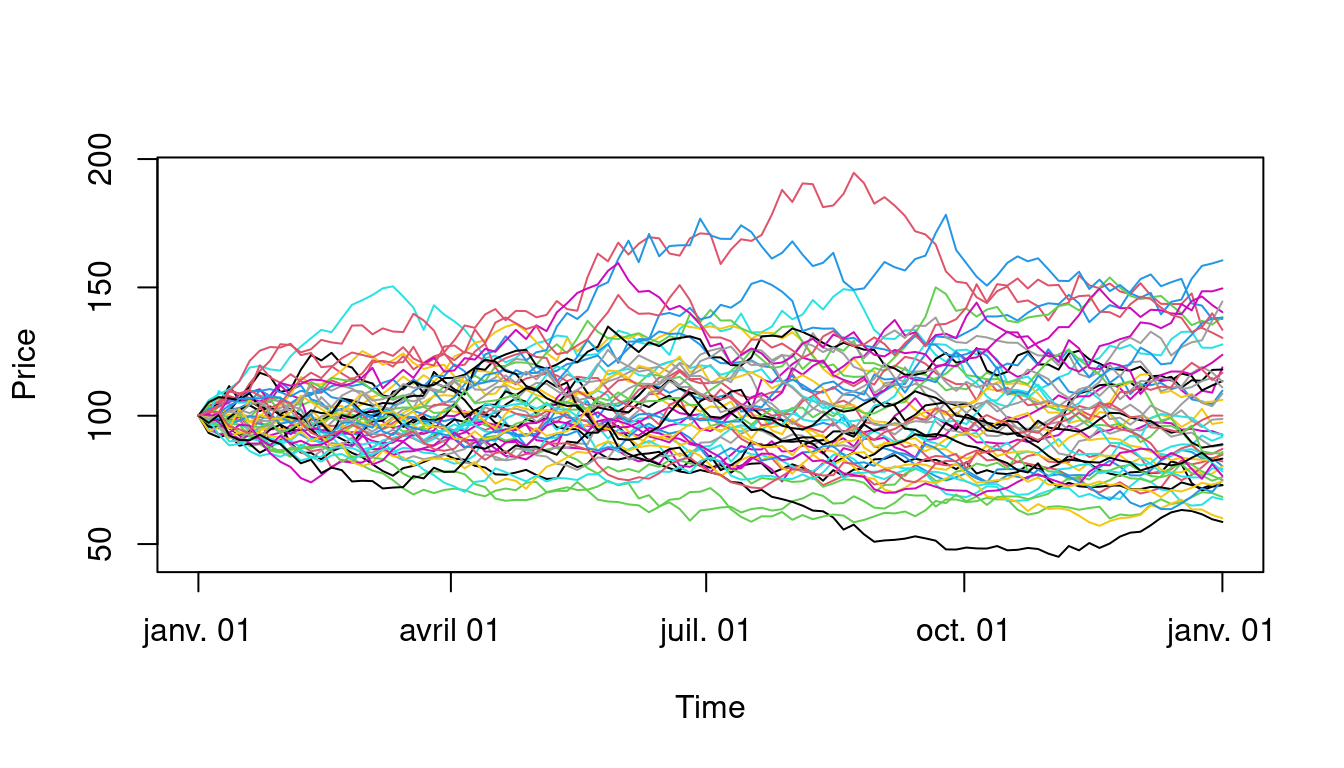
\includegraphics{empiricalfin_files/figure-latex/price-plot-1} \caption[Simulated price paths under a log-normal diffusion process]{Simulated price paths under a log-normal diffusion process}\label{fig:price-plot}
\end{marginfigure}

\hypertarget{a-delta-hedging-experiment}{%
\section{A Delta Hedging Experiment}\label{a-delta-hedging-experiment}}

Having generated some scenarios for the stock price, let's now simulate
the dynamic hedging of a European call option written on this stock,
using the Black-Scholes pricing model, with the implied volatility and
interest rate held constant.

Fist, we define the instrument to be hedged:

\begin{Shaded}
\begin{Highlighting}[]
\NormalTok{dtExpiry }\OtherTok{\textless{}{-}}\NormalTok{ dtEnd}

\NormalTok{underlying }\OtherTok{\textless{}{-}} \StringTok{"IBM"}
\NormalTok{K }\OtherTok{\textless{}{-}} \DecValTok{100}

\NormalTok{a }\OtherTok{\textless{}{-}} \FunctionTok{fInstrumentFactory}\NormalTok{(}\StringTok{"vanilla"}\NormalTok{, }\AttributeTok{quantity =} \DecValTok{1}\NormalTok{, }\AttributeTok{params =} \FunctionTok{list}\NormalTok{(}\AttributeTok{cp =} \StringTok{"c"}\NormalTok{,}
    \AttributeTok{strike =}\NormalTok{ K, }\AttributeTok{dtExpiry =}\NormalTok{ dtExpiry, }\AttributeTok{underlying =}\NormalTok{ underlying,}
    \AttributeTok{discountRef =} \StringTok{"USD.LIBOR"}\NormalTok{, }\AttributeTok{trace =} \ConstantTok{FALSE}\NormalTok{))}
\end{Highlighting}
\end{Shaded}

Next, we define the market data that will be held constant during the
simulation, and insert it in a \class{DataProvider}:

\begin{Shaded}
\begin{Highlighting}[]
\NormalTok{base.env }\OtherTok{\textless{}{-}} \FunctionTok{DataProvider}\NormalTok{()}
\FunctionTok{setData}\NormalTok{(base.env, underlying, }\StringTok{"Price"}\NormalTok{, dtStart, }\DecValTok{100}\NormalTok{)}
\FunctionTok{setData}\NormalTok{(base.env, underlying, }\StringTok{"DivYield"}\NormalTok{, dtStart,}
    \FloatTok{0.02}\NormalTok{)}
\FunctionTok{setData}\NormalTok{(base.env, underlying, }\StringTok{"ATMVol"}\NormalTok{, dtStart, sigma)}
\FunctionTok{setData}\NormalTok{(base.env, underlying, }\StringTok{"discountRef"}\NormalTok{, dtStart,}
    \StringTok{"USD.LIBOR"}\NormalTok{)}
\FunctionTok{setData}\NormalTok{(base.env, }\StringTok{"USD.LIBOR"}\NormalTok{, }\StringTok{"Yield"}\NormalTok{, dtStart, }\FloatTok{0.02}\NormalTok{)}
\end{Highlighting}
\end{Shaded}

At this stage, we can price the asset as of the start date of the
simulation:

\begin{Shaded}
\begin{Highlighting}[]
\NormalTok{p }\OtherTok{\textless{}{-}} \FunctionTok{getValue}\NormalTok{(a, }\StringTok{"Price"}\NormalTok{, dtStart, base.env)}
\end{Highlighting}
\end{Shaded}

which gives a value of \(p = 12.82\).

Next, define the simulation parameters: we want to simulate a dynamic
hedging policy over 500 paths, and 100 time steps per path:

We use a child \class{DataProvider} to store the simulated paths. Data not found in the child \class{DataProvider}
will be searched for (and found) in the parent \code{base.env}.

\begin{Shaded}
\begin{Highlighting}[]
\NormalTok{sce.env }\OtherTok{\textless{}{-}} \FunctionTok{DataProvider}\NormalTok{(}\AttributeTok{parent =}\NormalTok{ base.env)}
\FunctionTok{setData}\NormalTok{(sce.env, underlying, }\StringTok{"Price"}\NormalTok{, }\FunctionTok{time}\NormalTok{(tSpot),}
    \FunctionTok{as.matrix}\NormalTok{(tSpot))}
\end{Highlighting}
\end{Shaded}

We can now run the delta-hedge strategy along each path:

\begin{Shaded}
\begin{Highlighting}[]
\NormalTok{assets }\OtherTok{=} \FunctionTok{list}\NormalTok{(a)}
\NormalTok{res }\OtherTok{\textless{}{-}} \FunctionTok{deltaHedge}\NormalTok{(assets, sce.env, }\AttributeTok{params =} \FunctionTok{list}\NormalTok{(}\AttributeTok{dtSim =} \FunctionTok{time}\NormalTok{(tSpot),}
    \AttributeTok{transaction.cost =} \DecValTok{0}\NormalTok{), }\AttributeTok{trace =} \ConstantTok{FALSE}\NormalTok{)}
\end{Highlighting}
\end{Shaded}

The result is a data structure that contains the residual wealth
(hedging error) per scenario and time step. The distribution of hedging
error at expiry is shown in Figure \ref{fig:delta-hedge-41}.

\begin{Shaded}
\begin{Highlighting}[]
\FunctionTok{hist}\NormalTok{(}\FunctionTok{tail}\NormalTok{(res}\SpecialCharTok{$}\NormalTok{wealth, }\DecValTok{1}\NormalTok{), }\DecValTok{50}\NormalTok{, }\AttributeTok{xlab =} \StringTok{"Residual wealth at expiry"}\NormalTok{,}
    \AttributeTok{main =} \StringTok{""}\NormalTok{)}
\end{Highlighting}
\end{Shaded}

\begin{marginfigure}
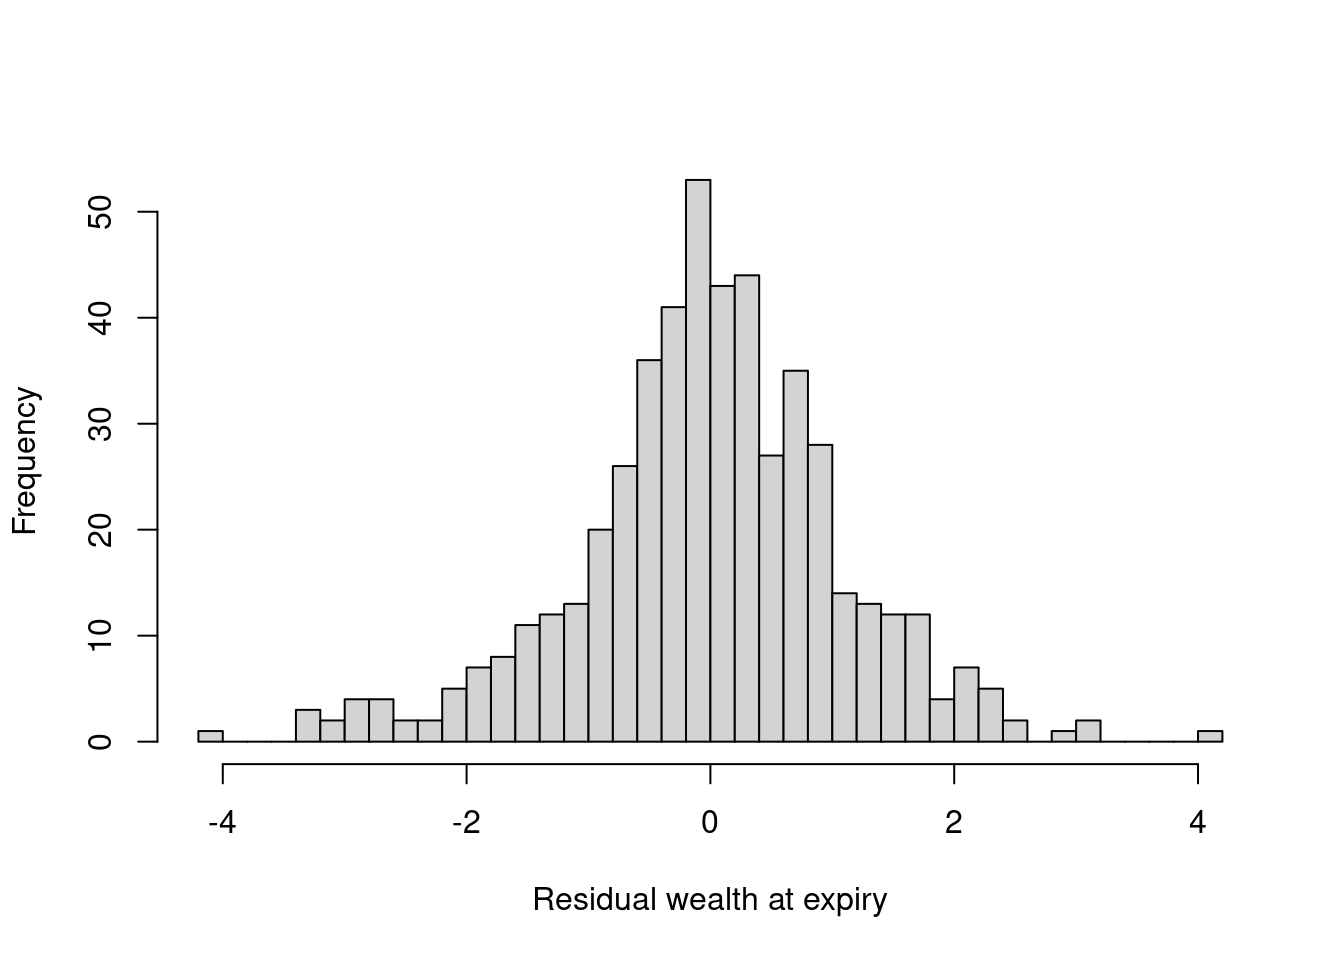
\includegraphics{empiricalfin_files/figure-latex/delta-hedge-41-1} \caption[Distribution of residual wealth at expiry]{Distribution of residual wealth at expiry: delta hedge of a 1 year call option}\label{fig:delta-hedge-41}
\end{marginfigure}

To better illustrate the hedging policy, let's run a toy example with
few time steps. The function \Rfun{deltaHedge} produces a detailed log of the hedging
policy, which is presented in Table \ref{tab:delta-hedge-few-samples}. For each time step,
the table show:

\begin{itemize}
\item
  The stock price,
\item
  the option delta,
\item
  the option value,
\item
  the value of the replicating portfolio and the short bond position in that portfolio.
\end{itemize}

\begin{Shaded}
\begin{Highlighting}[]
\NormalTok{dtSim }\OtherTok{\textless{}{-}} \FunctionTok{time}\NormalTok{(tSpot)[}\FunctionTok{seq}\NormalTok{(}\DecValTok{1}\NormalTok{, }\FunctionTok{dim}\NormalTok{(tSpot)[}\DecValTok{1}\NormalTok{], }\DecValTok{10}\NormalTok{)]}
\NormalTok{res }\OtherTok{\textless{}{-}} \FunctionTok{deltaHedge}\NormalTok{(assets, sce.env, }\AttributeTok{params =} \FunctionTok{list}\NormalTok{(}\AttributeTok{dtSim =}\NormalTok{ dtSim,}
    \AttributeTok{transaction.cost =} \DecValTok{0}\NormalTok{), }\AttributeTok{trace =} \ConstantTok{FALSE}\NormalTok{)}
\NormalTok{sim.table }\OtherTok{\textless{}{-}} \FunctionTok{makeTable}\NormalTok{(}\DecValTok{1}\NormalTok{, res)}
\end{Highlighting}
\end{Shaded}

\begin{table}

\caption{\label{tab:delta-hedge-few-samples}Simulated value of a call option and its hedge portfolio over time}
\centering
\begin{tabular}[t]{rrrrrr}
\toprule
time & stock price & delta & option & bond pos & hedge port.\\
\midrule
1 & 100.00000 & 0.5857659 & 12.8215847 & -46.679318 & 12.8215847\\
2 & 97.00535 & 0.5393194 & 10.4505725 & -42.091929 & 10.9758209\\
3 & 104.71501 & 0.6426285 & 14.2776535 & -53.084419 & 15.0510232\\
4 & 105.29617 & 0.6505785 & 13.8692900 & -53.933323 & 15.3199039\\
5 & 115.98565 & 0.7898772 & 20.7809251 & -70.285023 & 22.1677804\\
\addlinespace
6 & 94.43981 & 0.4536390 & 6.0882182 & -38.211619 & 5.0101741\\
7 & 97.30819 & 0.4972939 & 6.5169379 & -42.493719 & 6.2356476\\
8 & 87.15693 & 0.2364152 & 1.8346996 & -19.619493 & 1.1030904\\
9 & 84.01967 & 0.1148928 & 0.5969689 & -9.368302 & 0.3223531\\
10 & 80.58910 & 0.0136819 & 0.0356091 & -1.195477 & -0.0904753\\
\addlinespace
11 & 74.32359 & 0.0000000 & 0.0000000 & -0.178588 & -0.1785880\\
\bottomrule
\end{tabular}
\end{table}

\hypertarget{design-considerations}{%
\subsection{Design Considerations}\label{design-considerations}}

Two design features are worth mentioning.

The generation of the scenarios is independent from the expression of
the dynamic trading strategies. Remember that every data element stored
in a \class{DataProvider} is a \class{timeSeries}. Since all the calculations on \class{fInstrument} are vectorized, there is no
difference between performing a calculation on a scalar, or performing a
simulation on multiple scenarios.

The second aspect is the use of parent/child relationships among
\class{DataProvider} objects. All the market data that is held constant in the simulation is
stored in the parent \class{DataProvider}. The data that changes from simulation to
simulation is stored in the child \class{DataProvider}, and this is the object that is
passed to the simulator. When a piece of data is requested from the
child \class{DataProvider}, the following logic is applied:

\begin{enumerate}
\def\labelenumi{\arabic{enumi}.}
\item
  First look for the data in the current \class{DataProvider} (the object passed as
  argument to the simulator)
\item
  if not found, look for the data in the parent \class{DataProvider}.
\item
  and so forth: the logic is recursive.
\end{enumerate}

This behavior is inherited from the built-in \class{environment}.

\hypertarget{references}{%
\chapter{References}\label{references}}

\hypertarget{refs}{}
\begin{CSLReferences}{1}{0}
\leavevmode\vadjust pre{\hypertarget{ref-Fowler1996}{}}%
Fowler, Martin. 1996. \emph{{Analysis Patterns: Reusable Object Models}}. Addison-Wesley.

\end{CSLReferences}


\printindex

\end{document}
